\begin{exercice*} 
    Un centre nautique doit réparer une voile. La voile a la forme du triangle $PMW$ ci-dessous.
    \begin{tikzpicture}[scale=0.7]        
        % \draw[help lines, color=black!30, dashed] (0,0) grid (6,10);
        \coordinate (P) at (1,1);
        \coordinate (M) at (1,9);
        \coordinate (C) at (1,8);
        \coordinate (W) at (4.5,3);
        \tkzDefPointBy[homothety=center P ratio 0.875](W)	\tkzGetPoint{T};        
        \tkzDrawSegment[ultra thick](P,M);
        \tkzDrawSegment[ultra thick](P,W);
        \tkzDrawSegment[ultra thick](M,W);
        \tkzDrawSegment[dashed, ultra thick](C,T);
        \tkzLabelPoints[above left](M);
        \tkzLabelPoints[above left](C);
        \tkzLabelPoints[below left](P);
        \tkzLabelPoints[below right](T);
        \tkzLabelPoints[right](W);
        \begin{scope}[dim style/.append style={red, dashed}, dim fence style/.style={red, dashed}]                
            \tkzDrawSegment[dim={\(\Lg[m]{4.20}\),10mm,sloped,above=1mm}](P,M);
            \tkzDrawSegment[dim={\(\Lg[m]{3.78}\),5mm,sloped,above=1mm}](P,C);
            \tkzDrawSegment[dim={\(\Lg[m]{3.40}\),5mm,sloped,above=1mm}](M,W);            
        \end{scope}
    \end{tikzpicture}

    \begin{enumerate}
        \item On souhaite coudre suivant le segment $[CT]$. En supposant $(CT)$ parallèle à $(MW)$,
         déterminer la longueur de cette couture.
        \item La couture terminée, on constate que $PT=\Lg[m]{2.07}$ et $PW=\Lg[m]{2.30}$.        
        Déterminer si la couture est effectivement parallèle au bord.
    \end{enumerate}
\end{exercice*}
\begin{corrige}
    %\setcounter{partie}{0} % Pour s'assurer que le compteur de \partie est à zéro dans les corrigés
    \phantom{rrr}

    \begin{multicols}{2}
        Un centre nautique doit réparer une voile. La voile a la forme du triangle $PMW$ ci-dessous.
        \begin{tikzpicture}[scale=0.5]        
            % \draw[help lines, color=black!30, dashed] (0,0) grid (6,10);
            \coordinate (P) at (1,1);
            \coordinate (M) at (1,9);
            \coordinate (C) at (1,8);
            \coordinate (W) at (4.5,3);
            \tkzDefPointBy[homothety=center P ratio 0.875](W)	\tkzGetPoint{T};        
            \tkzDrawSegment[ultra thick](P,M);
            \tkzDrawSegment[ultra thick](P,W);
            \tkzDrawSegment[ultra thick](M,W);
            \tkzDrawSegment[dashed, ultra thick](C,T);
            \tkzLabelPoints[above left](M);
            \tkzLabelPoints[above left](C);
            \tkzLabelPoints[below left](P);
            \tkzLabelPoints[below right](T);
            \tkzLabelPoints[right](W);
            \begin{scope}[dim style/.append style={red, dashed}, dim fence style/.style={red, dashed}]                
                \tkzDrawSegment[dim={\(\Lg[m]{4.20}\),10mm,sloped,above=1mm}](P,M);
                \tkzDrawSegment[dim={\(\Lg[m]{3.78}\),5mm,sloped,above=1mm}](P,C);
                \tkzDrawSegment[dim={\(\Lg[m]{3.40}\),5mm,sloped,above=1mm}](M,W);            
            \end{scope}
        \end{tikzpicture}
    
        \begin{enumerate}
            \item On souhaite coudre suivant le segment $[CT]$. En supposant $(CT)$ parallèle à $(MW)$,
             déterminer la longueur de cette couture.

             {\color{red}
                \Thales[Droites,Unite=m]{PMWCT}{PT}{3.78}{CT}{PW}{4.2}{3.40}             
             }
            \item La couture terminée, on constate que $PT=\Lg[m]{2.07}$ et $PW=\Lg[m]{2.30}$.        
            Déterminer si la couture est effectivement parallèle au bord.

            {\color{red}
                % \Thales[Reciproque,Simplification=false]{PMWCT}{3.78}{4.2}{2.07}{2.30}{}{}
                \Thales[Reciproque,Droites,Produit]{PMWCT}{3.78}{4.2}{2.07}{2.3}{100}{100}
            }
        \end{enumerate}
    \end{multicols}

\end{corrige}

